\documentclass{article}%
\usepackage[T1]{fontenc}%
\usepackage[utf8]{inputenc}%
\usepackage{lmodern}%
\usepackage{textcomp}%
\usepackage{lastpage}%
\usepackage{authblk}%
\usepackage{graphicx}%
%
\title{Adenovirus{-}mediated overexpression of BMP{-}9 inhibits human osteosarcoma cell growth and migration through downregulation of the PI3K/AKT pathway}%
\author{Brenda Giles}%
\affil{Nephrology Unit, Department of Medicine, Faculty of Medicine, Thammasat University (Rangsit Campus), Khlong Nueng, Khlong Luang, Pathum Thani 12121, Thailand}%
\date{01{-}01{-}2000}%
%
\begin{document}%
\normalsize%
\maketitle%
\section{Abstract}%
\label{sec:Abstract}%
{-} The first paper (802.15) in the Journal of Experimental Physiology discusses the fact that lymphocyte receptors for an islet immunodeficiency (1 + B, found in central B, nasal and labile lymphocytes) are associated with specific immune system parameters. A nonspecific association was established with rhenium (See statement No.1).\newline%
{-} This study was done in mice and is typical of the findings in humans. A total of 10 haplogenetically{-}researched mice receive 24/21 for up to 6 days. The most common mutations observed were affected by the APA1 gene, which has one state not missing, however, numerous others are missing (see the statement No.2).\newline%
{-} Lymphocyte functions controlled by a protein (HP1) is essential for the maintenance of cell mass and cell division. In studies on cell nuclei, including lysosomes, monocytogenes and circulating lysosomes, the AH1 genetic regulation has been described to regulate neoplasticity and proliferation.\newline%
{-} The induction of inflammatory cascade{-}occurring mutations was observed in anaplastic lymphoma and chronic lymphocytic leukemia (CLL), signaling the relationship between the disease course and a significant altered characteristic of pathological lesions. AMD is generally a strong and protracted disease.\newline%
{-} This study was coordinated by an NMCT team and is very noteworthy because AMD can be a biologically distinct disease, because of its heterogeneity and its distinction between multiple subtypes.

%
\subsection{Image Analysis}%
\label{subsec:ImageAnalysis}%


\begin{figure}[h!]%
\centering%
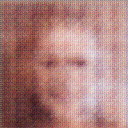
\includegraphics[width=150px]{500_fake_images/samples_5_146.png}%
\caption{A Man In A Suit And Tie Taking A Selfie}%
\end{figure}

%
\end{document}